\documentclass[12pt,a4paper]{article}
\usepackage[margin=1in]{geometry}
\usepackage{graphicx}
\usepackage{float}
\usepackage{booktabs}
\usepackage{array}
\usepackage{enumitem}
\usepackage{fancyhdr}
\usepackage{hyperref}
\usepackage{xcolor}

\graphicspath{{../screenshots/}{./}}
\hypersetup{colorlinks=true,linkcolor=blue,urlcolor=blue}
\pagestyle{fancy}
\fancyhf{}
\lhead{E-Commerce Website Automation}
\rhead{Sayan Dey}
\cfoot{\thepage}
\setlength{\headheight}{15pt}

\begin{document}

% 1. Title Page
\begin{titlepage}
\centering
\vspace*{1.1cm}
{\Huge\bfseries E-Commerce Website Automation\par}
\vspace{0.35cm}
{\Large Selenium WebDriver Capstone Project Report\par}
\vspace{1cm}
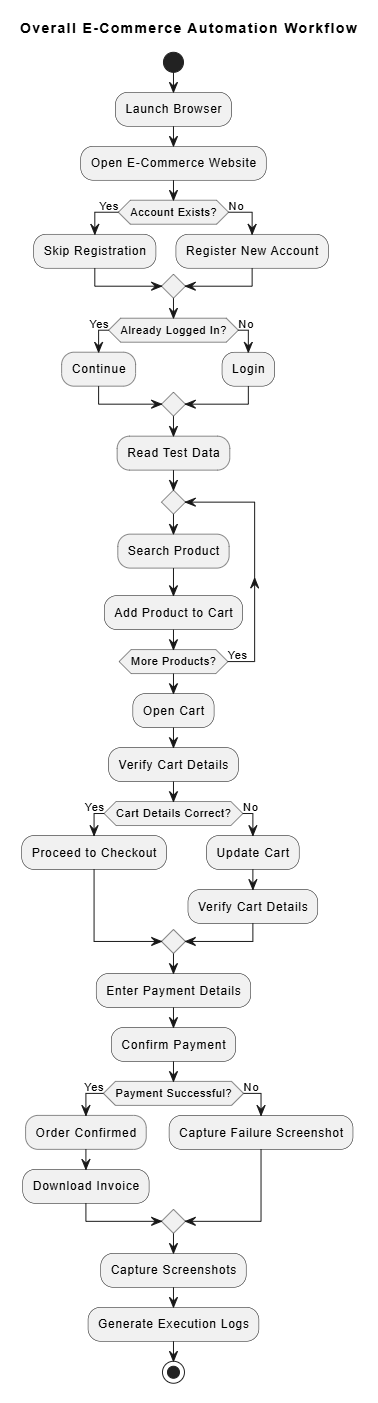
\includegraphics[width=0.88\textwidth,height=0.52\textheight,keepaspectratio]{flowchart.png}\par
\vspace{0.5cm}
{\large Overall Automation Workflow\par}
\vfill
{\Large\bfseries Author: Sayan Dey\par}
\vspace{0.3cm}
{\large \today\par}
\end{titlepage}

% 2. Abstract
\section*{2. Abstract}
\addcontentsline{toc}{section}{2. Abstract}
This report presents an end-to-end e-commerce website automation project built with Python, Selenium WebDriver, Firefox, and Pytest. The automated scenario opens the Automation Exercise website, registers or reuses a test account, signs in when needed, searches a data-driven product list, adds products to the cart, proceeds through checkout, enters test payment data, and records the final confirmation state. The project separates account, search, cart, logging, and screenshot responsibilities into focused modules. Explicit waits, exception logging, CSV test data, and screenshot evidence are used to make the workflow repeatable and easier to diagnose.

\tableofcontents
\clearpage
\setcounter{section}{2}

% 3. Introduction
\section{Introduction}
Modern e-commerce systems require reliable validation of complete customer journeys, not only isolated page actions. A simple failure in login, product search, cart handling, or checkout can prevent a customer from completing a purchase. This project automates that business-critical journey on the Automation Exercise demo website.

The project is a browser-based UI automation exercise. It uses a single Firefox session to maintain authentication and cart state from the landing page through payment confirmation. The main Pytest scenario is implemented in \texttt{test\_ecommerce.py}; \texttt{launch.py} provides a standalone runner for the same high-level sequence. The output of a successful run includes logs and screenshots that show the major application states.

% 4. Problem Statement
\section{Problem Statement}
Manual validation of an e-commerce purchase flow is repetitive, slow, and susceptible to human oversight. It requires repeated account setup, product discovery, form completion, cart navigation, and payment submission. Changes in page timing or dynamic content can also make manual checks inconsistent.

The problem addressed by this project is how to create a repeatable automated test that validates the main online-shopping workflow from account access to order completion. The solution must handle existing accounts, dynamic page elements, multiple products, and evidence collection while remaining understandable and maintainable.

% 5. Objectives
\section{Objectives}
\begin{itemize}[leftmargin=1.6em]
  \item Automate registration, login, product search, cart addition, checkout, payment, and order completion.
  \item Read test inputs from configuration and CSV files instead of hard-coding product and account data in the test flow.
  \item Use Selenium explicit waits to synchronize browser actions with page readiness.
  \item Capture visual evidence at important stages and write execution details to a log file.
  \item Organize code into reusable modules for account, search, cart, and utility tasks.
\end{itemize}

% 6. Technologies Used
\section{Technologies Used}
\begin{table}[H]
\centering
\begin{tabular}{p{0.30\textwidth}p{0.58\textwidth}}
\toprule
\textbf{Technology} & \textbf{Use in the Project} \\
\midrule
Python & Primary implementation language for the automation scripts. \\
Selenium WebDriver & Browser automation API used to control Firefox and interact with the web application. \\
Pytest & Test runner and fixture framework for the end-to-end scenario. \\
Mozilla Firefox & Browser used by the WebDriver session. \\
CSV / ConfigParser & External test data and application URL configuration. \\
Python logging & Timestamped execution and failure messages in \texttt{log.txt}. \\
LaTeX and MiKTeX & Report preparation and PDF compilation. \\
\bottomrule
\end{tabular}
\caption{Technologies used in the project.}
\end{table}

% 7. System Requirements
\section{System Requirements}
The project requires a Windows system with Python 3.10 or later, Mozilla Firefox, Selenium 4, Pytest, network access to \url{https://automationexercise.com/}, and a compatible Firefox WebDriver environment. Modern Selenium versions can manage the driver automatically when the local browser environment is supported; otherwise GeckoDriver must be available on the system path. To compile this report, MiKTeX with \texttt{pdflatex} is required.

The test uses the source files \texttt{config.ini}, \texttt{testdata.csv}, and \texttt{products.csv}. The browser needs permission to create or overwrite PNG files in the \texttt{screenshots} folder and append runtime information to \texttt{log.txt}.

% 8. Project Architecture
\section{Project Architecture}
The architecture is a modular functional design. The test runner owns the browser lifetime and orchestrates the business sequence. Domain modules receive the shared Selenium \texttt{driver} instance, allowing the same session, authenticated user, and cart contents to persist throughout the run. The full workflow diagram is presented on the title page.

The data layer contains the application URL in \texttt{config.ini}, customer details in \texttt{testdata.csv}, and products in \texttt{products.csv}. The support layer contains screenshot capture and logging. This separation makes it possible to update input data without rewriting the full workflow.

% 9. Project Workflow
\section{Project Workflow}
The workflow begins by starting Firefox and opening the configured URL. Registration reads the first test-data record and attempts to create an account. If the account-information form is unavailable after signup, the email is treated as already registered and registration is skipped. Login then checks whether a Logout link exists; if not, it signs in with CSV credentials and waits for the logged-in indicator.

The test reads every product row, searches for the exact product name, adds the matching item to the cart, and continues shopping until all products have been processed. It then opens the cart, proceeds to checkout, places the order, submits test card values, waits for a page transition from the payment URL, and captures the order-success screenshot. Finally, the browser is closed by fixture teardown or the standalone runner's \texttt{finally} block.

% 10. Project Structure
\section{Project Structure}
\begin{table}[H]
\centering
\small
\begin{tabular}{p{0.30\textwidth}p{0.58\textwidth}}
\toprule
\textbf{File or Folder} & \textbf{Purpose} \\
\midrule
\texttt{test\_ecommerce.py} & Pytest fixture and complete end-to-end test scenario. \\
\texttt{launch.py} & Standalone runner for the same business workflow. \\
\texttt{register.py}, \texttt{login.py} & Account creation and authentication. \\
\texttt{search.py} & Products-page navigation, product search, and result check. \\
\texttt{cart.py} & Add-to-cart, cart view, checkout, order placement, and payment. \\
\texttt{screenshot.py}, \texttt{logger.py} & Screenshot creation and centralized logging. \\
\texttt{popup.py} & Optional advertisement-iframe removal helper. \\
\texttt{products.csv}, \texttt{testdata.csv} & Product and customer test data. \\
\texttt{screenshots/} & Evidence images produced during execution. \\
\texttt{Report/} & Flowchart source, flowchart image, and this report. \\
\bottomrule
\end{tabular}
\caption{Project file structure.}
\end{table}

% 11. Test Automation Framework
\section{Test Automation Framework}
Pytest is used as the test automation framework. The \texttt{driver} fixture creates Firefox, configures it with eager page loading and image loading disabled, opens the target website, and yields the ready driver to \texttt{test\_ecommerce\_flow}. After the test completes or fails, the fixture closes the browser.

The standalone \texttt{launch.py} runner performs similar setup through helper functions and uses \texttt{try/except/finally} to ensure driver cleanup. The Pytest runner is preferable for repeatable automated execution because fixtures provide a clear setup and teardown boundary.

% 12. Selenium WebDriver
\section{Selenium WebDriver}
Selenium WebDriver controls Firefox through \texttt{webdriver.Firefox}. The driver opens URLs, locates page elements, fills forms, selects dropdown values, clicks controls, executes JavaScript scrolling, reads the current URL, and saves browser screenshots.

The cart module demonstrates several WebDriver capabilities: it locates a product card, scrolls the Add to Cart link to the center of the viewport, clicks it, waits for the confirmation modal, and continues shopping. Registration uses Selenium's \texttt{Select} helper for date-of-birth and country dropdowns. Payment automation enters the site's test card data and waits until the browser leaves the payment page.

% 13. Web Element Locators
\section{Web Element Locators}
The project uses a combination of locator strategies selected according to the structure of the target page:
\begin{itemize}[leftmargin=1.6em]
  \item \textbf{CSS selectors}: stable \texttt{data-qa} fields such as login email, signup button, payment inputs, and checkout links.
  \item \textbf{IDs}: direct identifiers such as \texttt{search\_product}, \texttt{submit\_search}, newsletter, and gender radio buttons.
  \item \textbf{Partial link text}: navigation controls including Products, Cart, Signup / Login, and Logout.
  \item \textbf{XPath}: exact product-name verification, parent product-card selection, modal controls, and text-based validation.
\end{itemize}
Using exact product text in the search result prevents the script from adding an unrelated result. The locator choices are encapsulated inside the modules, reducing their impact on the orchestration code.

% 14. Page Object Model (POM)
\section{Page Object Model (POM)}
The project does not currently implement a formal class-based Page Object Model. Instead, it uses a functional modular approach: \texttt{register.py}, \texttt{login.py}, \texttt{search.py}, and \texttt{cart.py} group actions by page or business area. This gives the project several POM-like benefits, including separation of locators from the central workflow and reusable page-level functions.

For a larger project, the next step would be to convert these modules into page classes such as \texttt{LoginPage}, \texttt{ProductsPage}, \texttt{CartPage}, and \texttt{PaymentPage}. Each class would store locators and expose business-focused methods. This would reduce duplication and improve maintainability if the website UI changes.

% 15. Test Case Design
\section{Test Case Design}
The main test case is an end-to-end positive purchase scenario. Preconditions are an available Automation Exercise website, Firefox, valid test data, and network access. The input products are Blue Top, Men Tshirt, and Sleeveless Dress. The expected outcome is that each product can be found and added, checkout can be reached, payment can be submitted, and navigation reaches an order-completion URL.

The scenario also includes decision paths for account state. A new email follows the registration route, while an existing email skips the rest of registration and moves to login. A pre-authenticated browser session bypasses login through the Logout-link check.

% 16. Test Execution
\section{Test Execution}
The test can be run with \texttt{python -m pytest -v test\_ecommerce.py}; the standalone flow can be executed with \texttt{python launch.py}. A recorded successful execution in \texttt{log.txt} processed three products, reached a \texttt{/payment\_done/} URL, logged a successful completion message, and closed Firefox.

\begin{figure}[H]
\centering
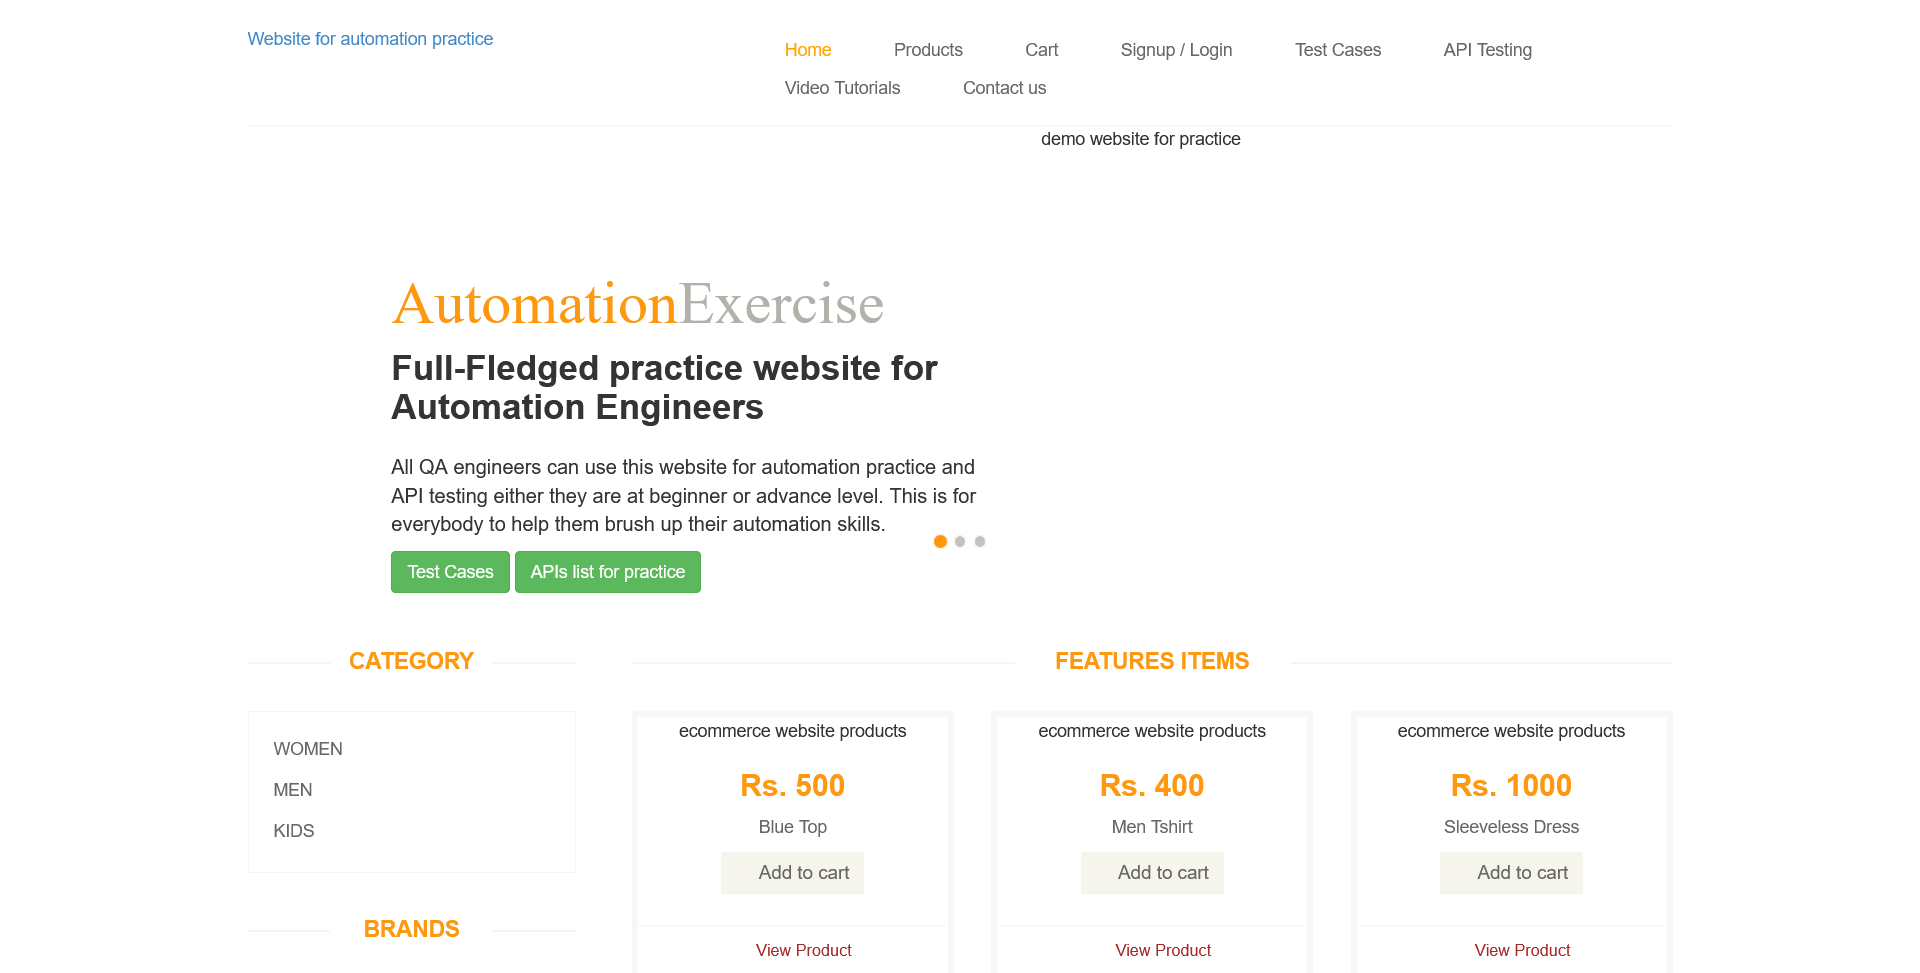
\includegraphics[width=0.80\textwidth]{01_homepage.png}
\caption{Homepage captured after browser initialization.}
\end{figure}

% 17. Synchronization and Wait Handling
\section{Synchronization and Wait Handling}
The automation primarily uses \texttt{WebDriverWait} with Selenium expected conditions rather than relying on arbitrary sleep delays. It waits for elements to become visible or clickable before interacting with navigation links, forms, search controls, modal buttons, and checkout actions. It also waits for the cart URL and for navigation away from the payment page.

This approach is more reliable than immediately attempting actions while the page is still changing. The one fixed delay in the Pytest test is only used to keep the browser visible briefly after the workflow; it is not used to decide whether a page element is ready.

% 18. Exception Handling
\section{Exception Handling}
Each workflow module surrounds its main operations with \texttt{try/except} blocks. When an operation fails, the code logs a descriptive message with the error and re-raises the exception so Pytest or the standalone runner reports a failed test. The standalone runner uses a \texttt{finally} block to call \texttt{driver.quit()} even after failure.

This design preserves the original failure signal while adding context to \texttt{log.txt}. A future improvement is to capture a failure screenshot automatically from every exception handler before re-raising the error.

% 19. Assertions and Validation
\section{Assertions and Validation}
The project currently validates progress through explicit conditions rather than Pytest \texttt{assert} statements. Examples include waiting for the ``Logged in as'' text, locating an exact matching product, confirming that the cart URL contains \texttt{/view\_cart}, confirming that the Account Created heading is visible for new accounts, and waiting until the payment URL changes after submission.

These checks provide meaningful validation points; however, the test can be strengthened by adding explicit assertions for product name, cart quantities, item totals, checkout address details, and an order-success message. The current \texttt{quantity} column in \texttt{products.csv} is not applied by the automation.

% 20. Test Results
\section{Test Results}
The available log and screenshots show a successful run. The account already existed, so registration was skipped; login succeeded; all three configured products were searched and added; the cart, checkout, and payment stages completed; and the final URL changed to an order-completion page. The following evidence images were produced by the test.

\begin{figure}[H]\centering
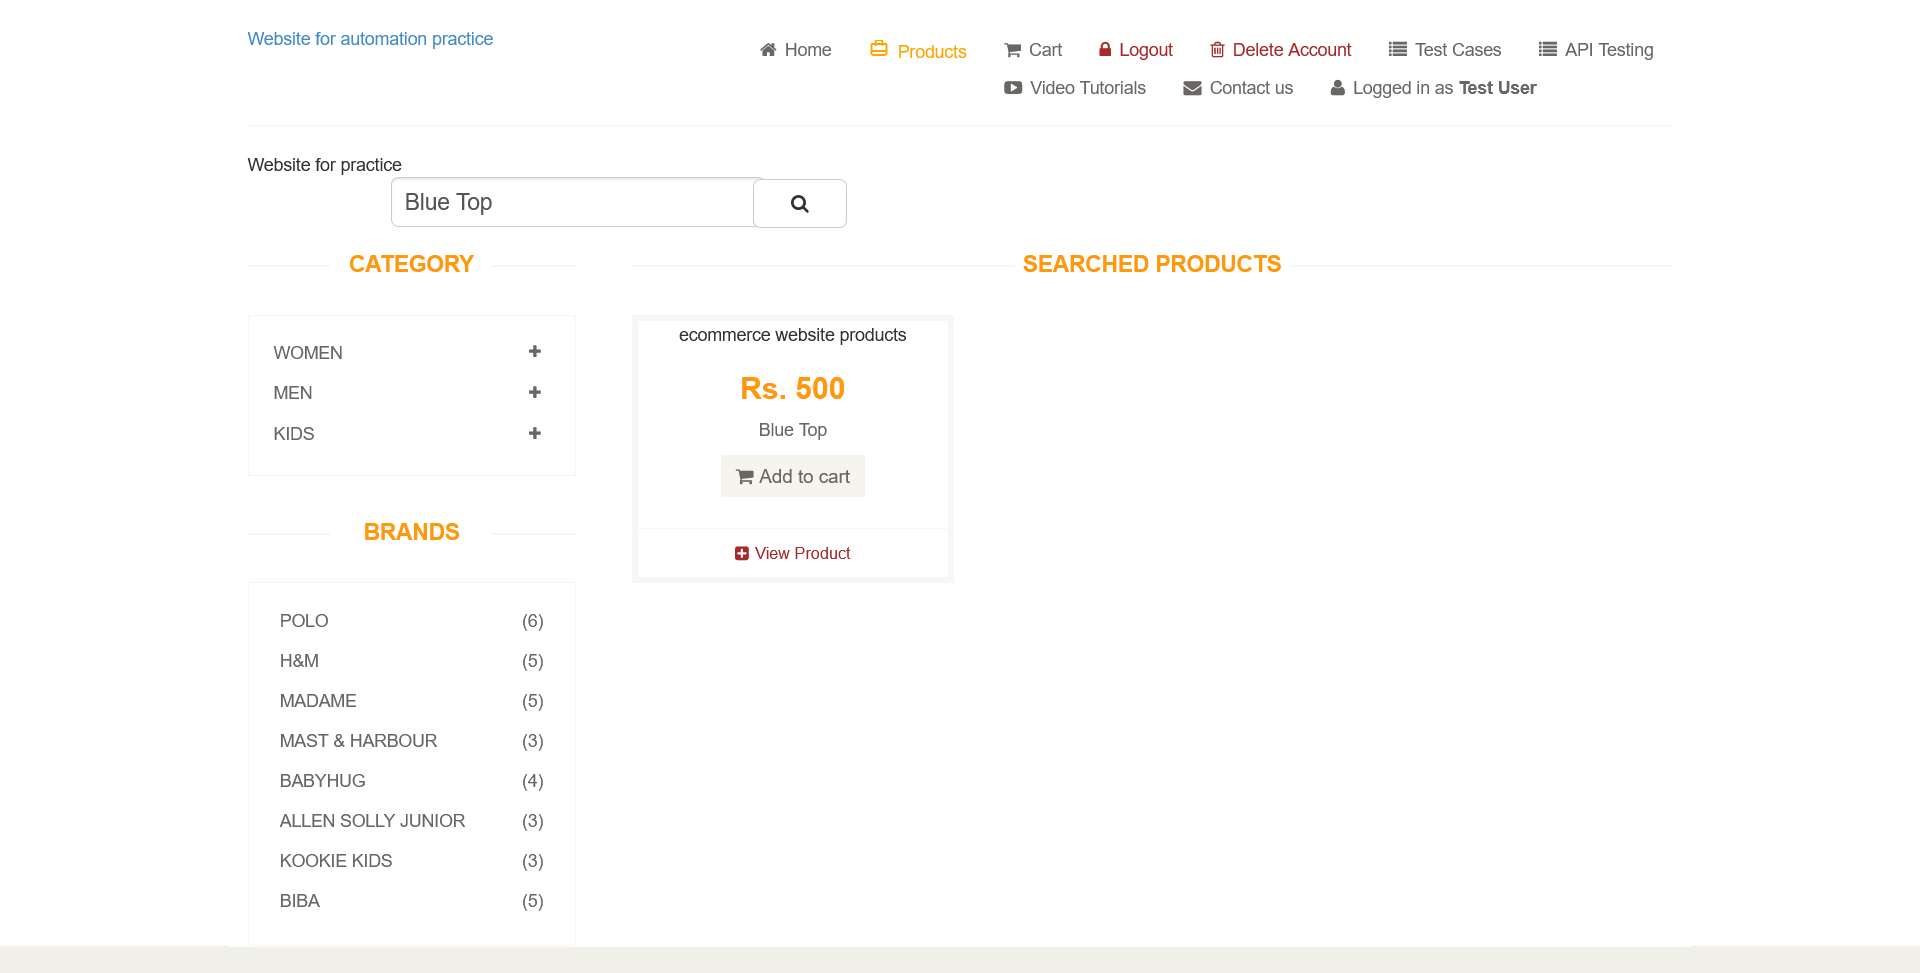
\includegraphics[width=0.68\textwidth]{add_to_cart_Blue_Top.png}
\caption{Blue Top located before cart addition.}
\end{figure}
\begin{figure}[H]\centering
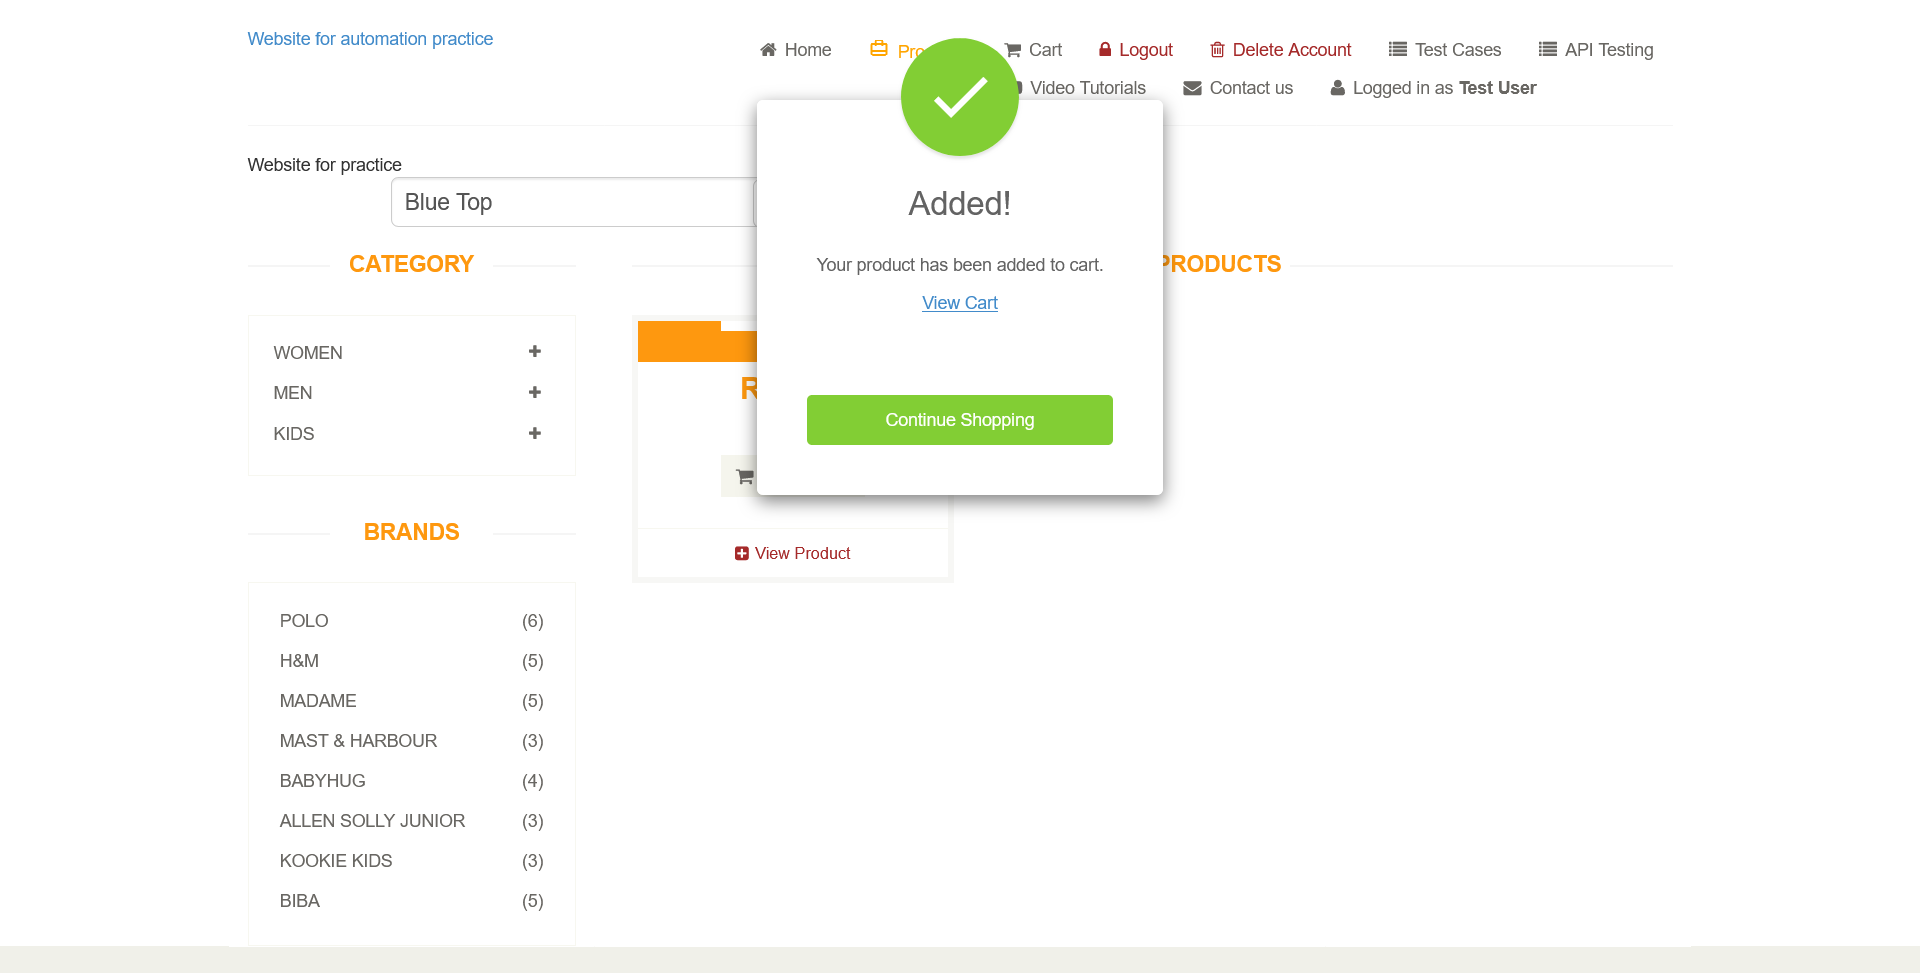
\includegraphics[width=0.68\textwidth]{cart_added_Blue_Top.png}
\caption{Blue Top added-to-cart confirmation.}
\end{figure}
\begin{figure}[H]\centering
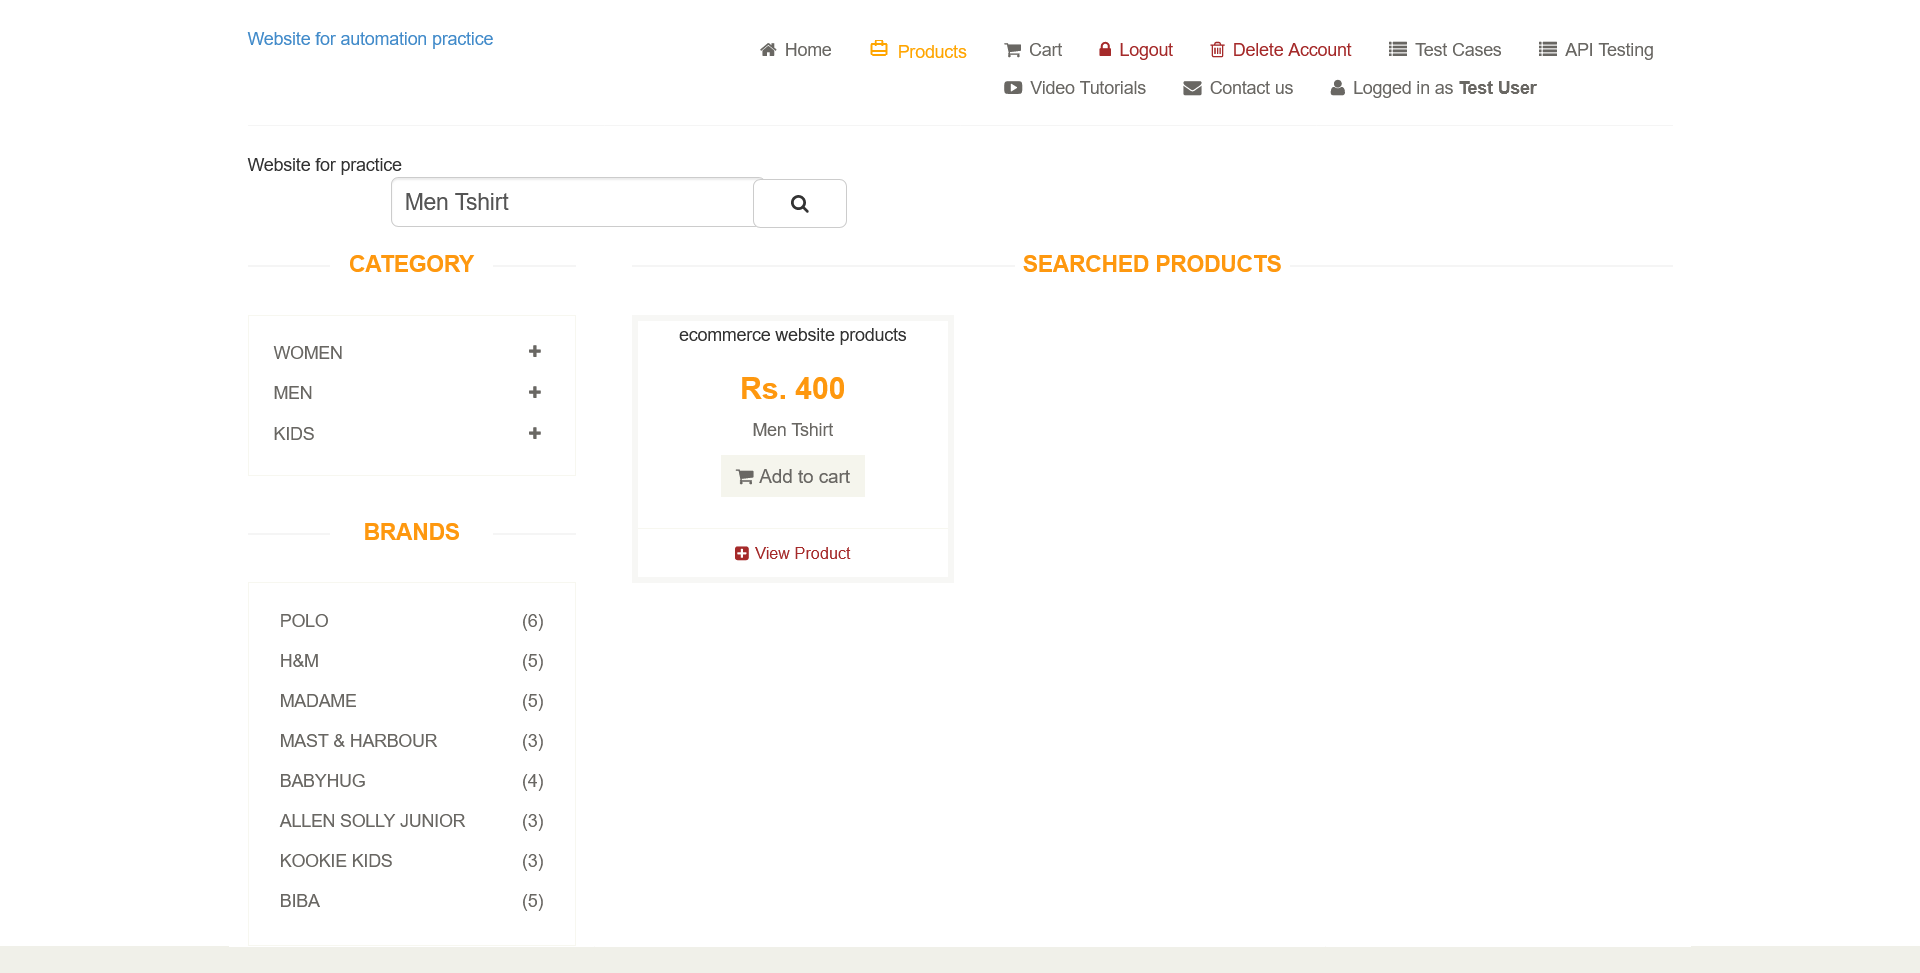
\includegraphics[width=0.68\textwidth]{add_to_cart_Men_Tshirt.png}
\caption{Men Tshirt located before cart addition.}
\end{figure}
\begin{figure}[H]\centering
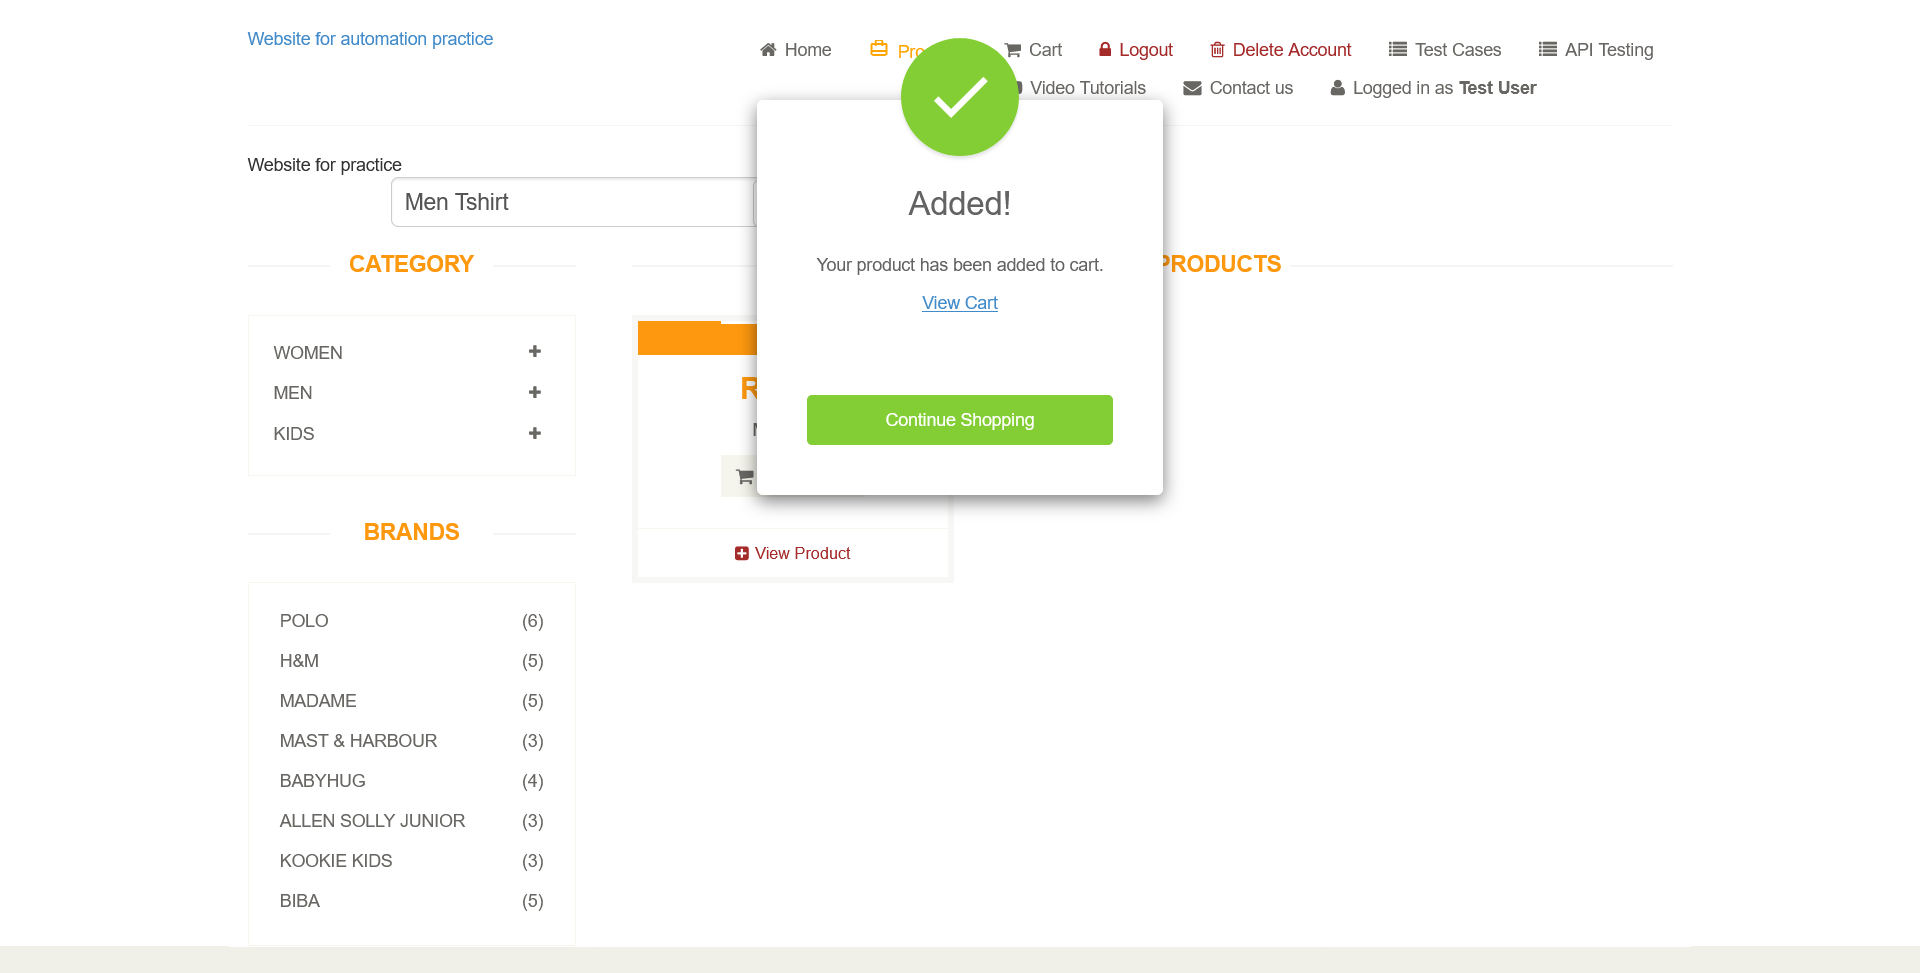
\includegraphics[width=0.68\textwidth]{cart_added_Men_Tshirt.png}
\caption{Men Tshirt added-to-cart confirmation.}
\end{figure}
\begin{figure}[H]\centering
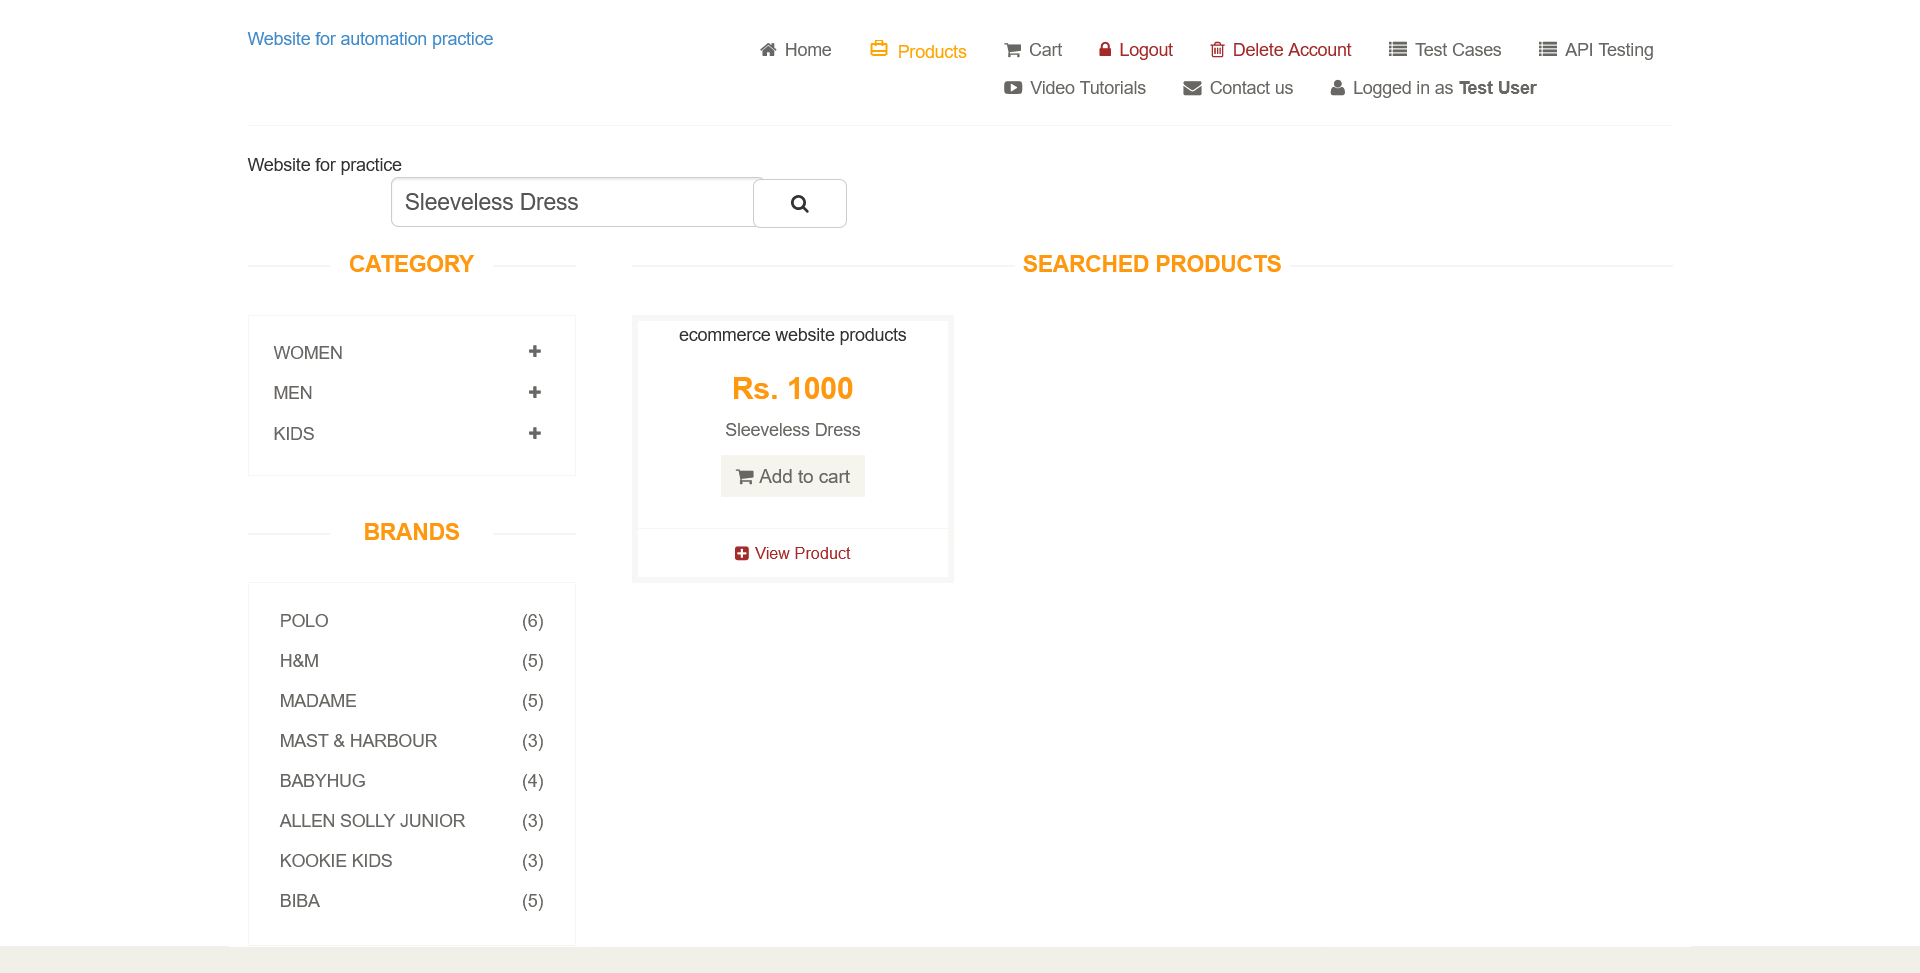
\includegraphics[width=0.68\textwidth]{add_to_cart_Sleeveless_Dress.png}
\caption{Sleeveless Dress located before cart addition.}
\end{figure}
\begin{figure}[H]\centering
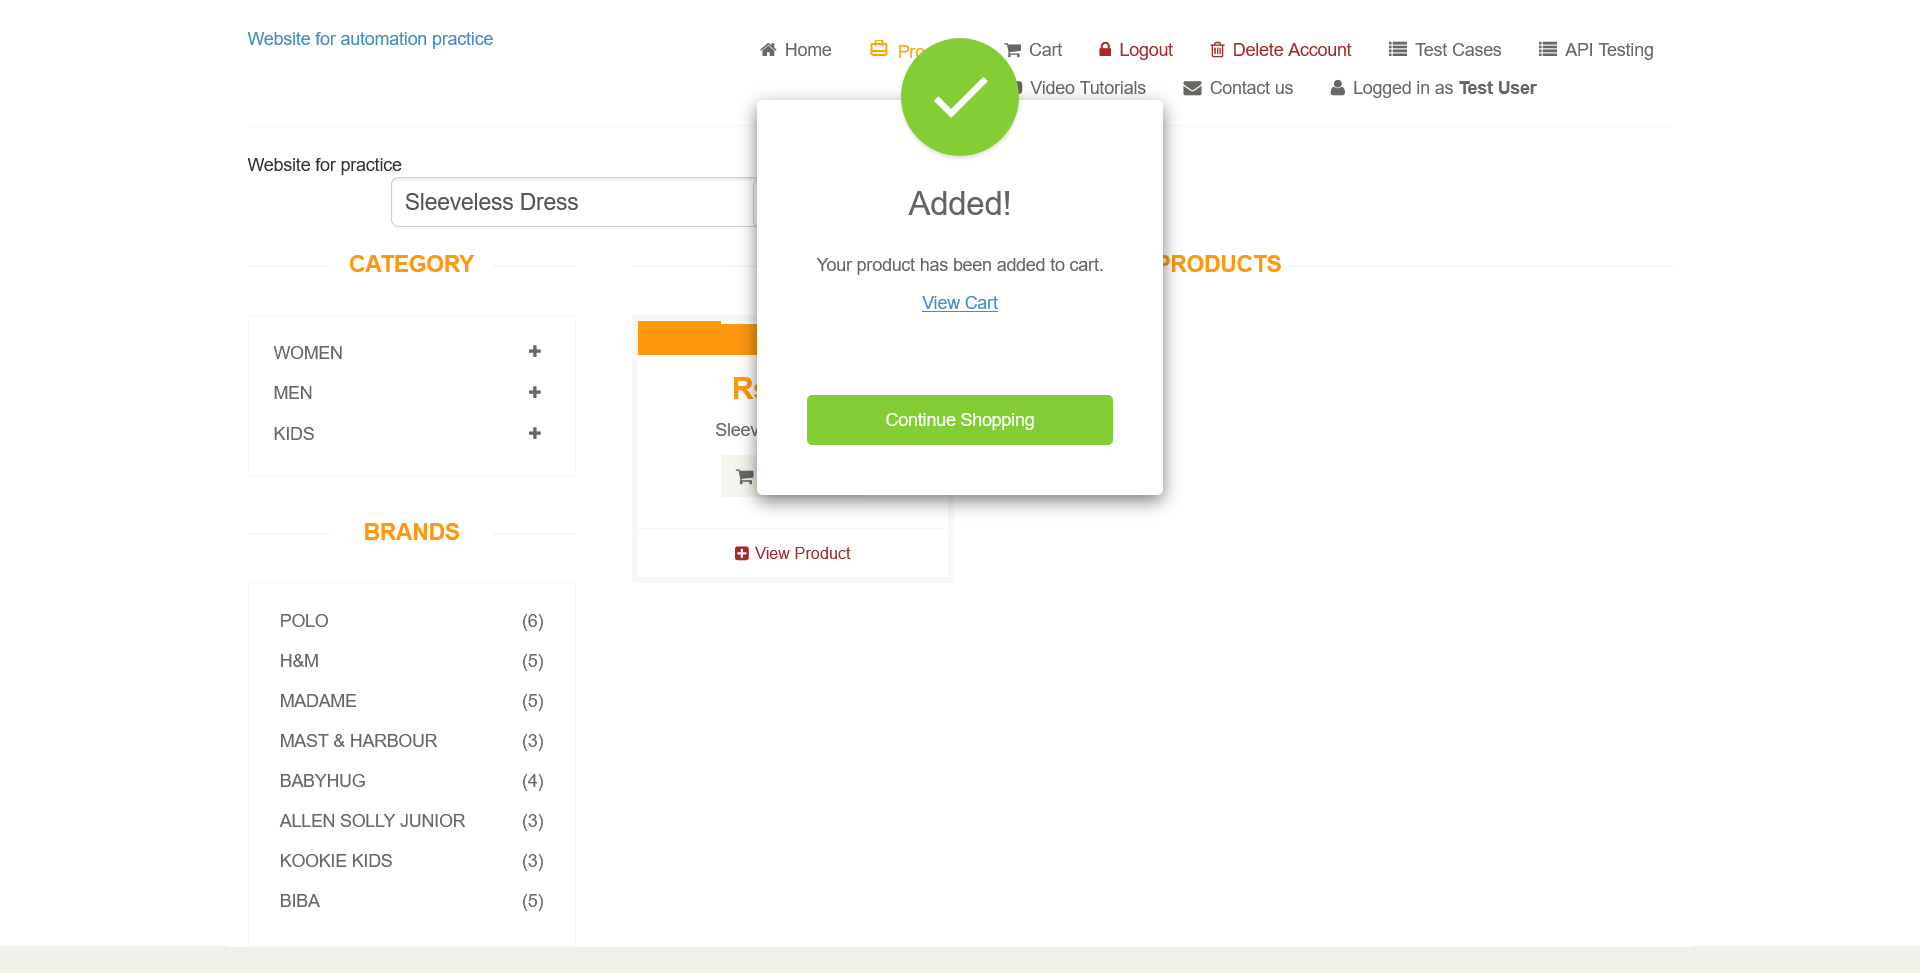
\includegraphics[width=0.68\textwidth]{cart_added_Sleeveless_Dress.png}
\caption{Sleeveless Dress added-to-cart confirmation.}
\end{figure}
\begin{figure}[H]\centering
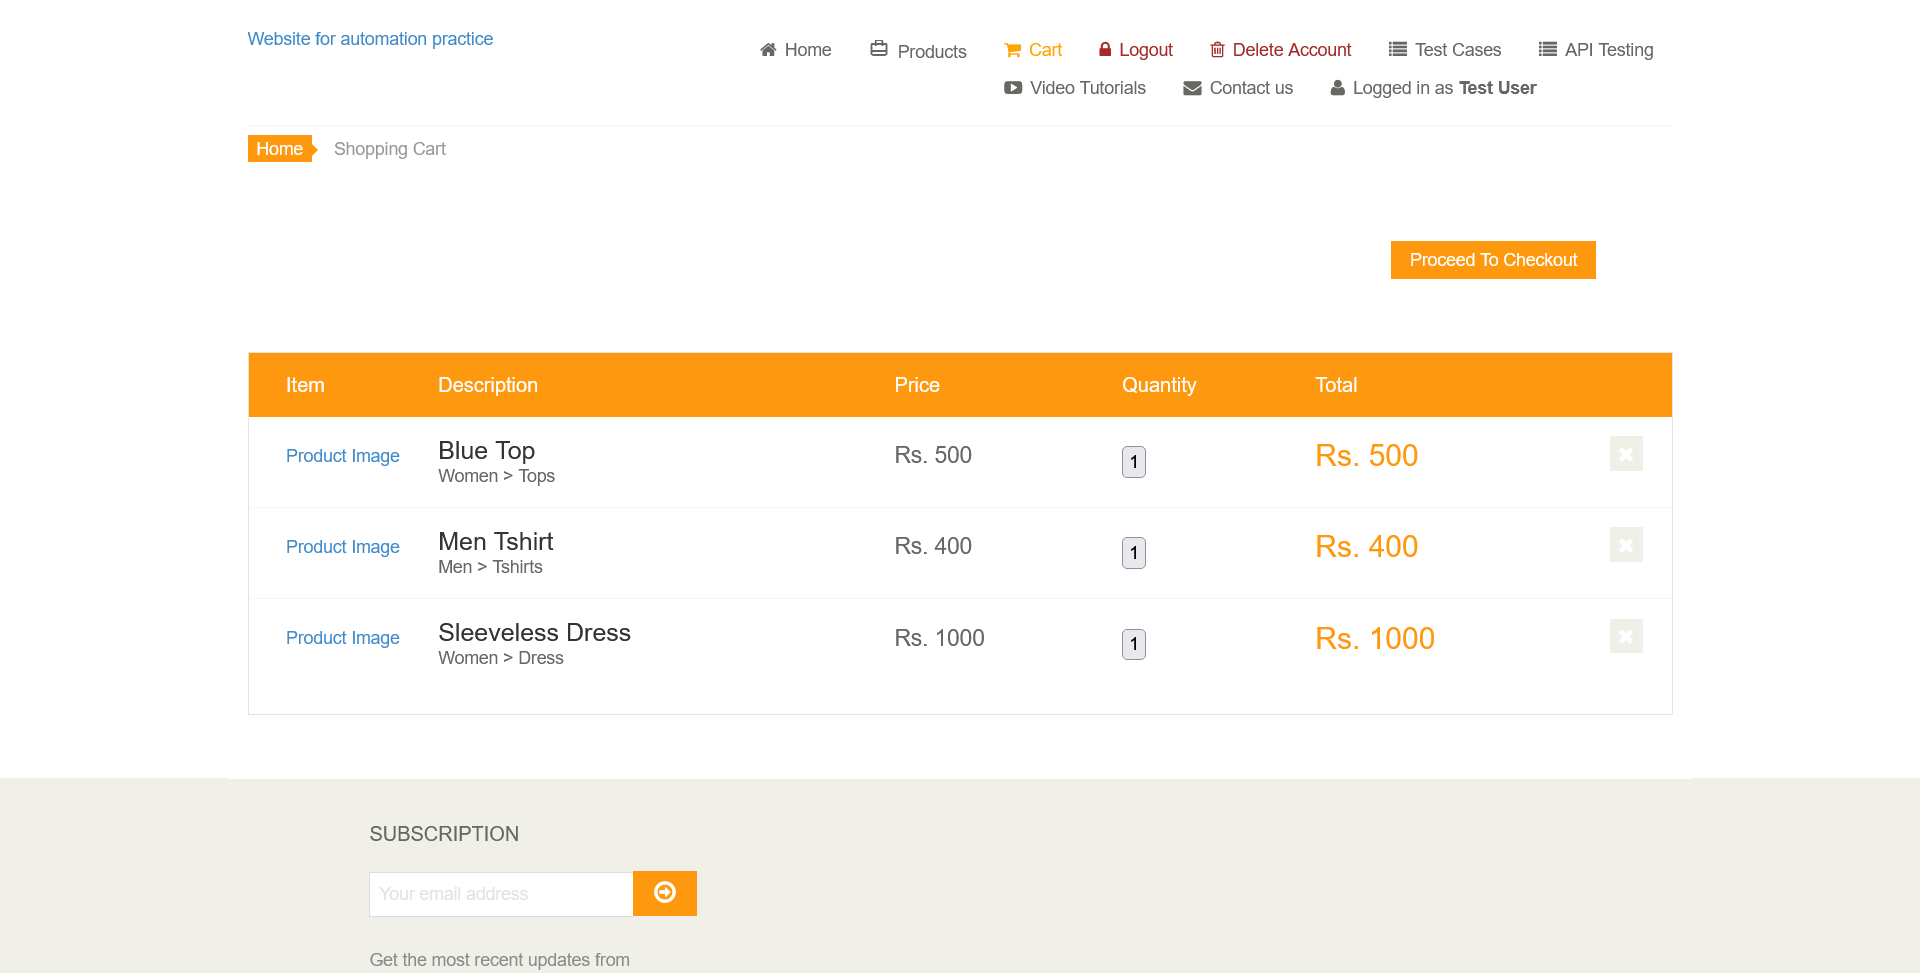
\includegraphics[width=0.76\textwidth]{cart_view.png}
\caption{Cart view after products were added.}
\end{figure}
\begin{figure}[H]\centering
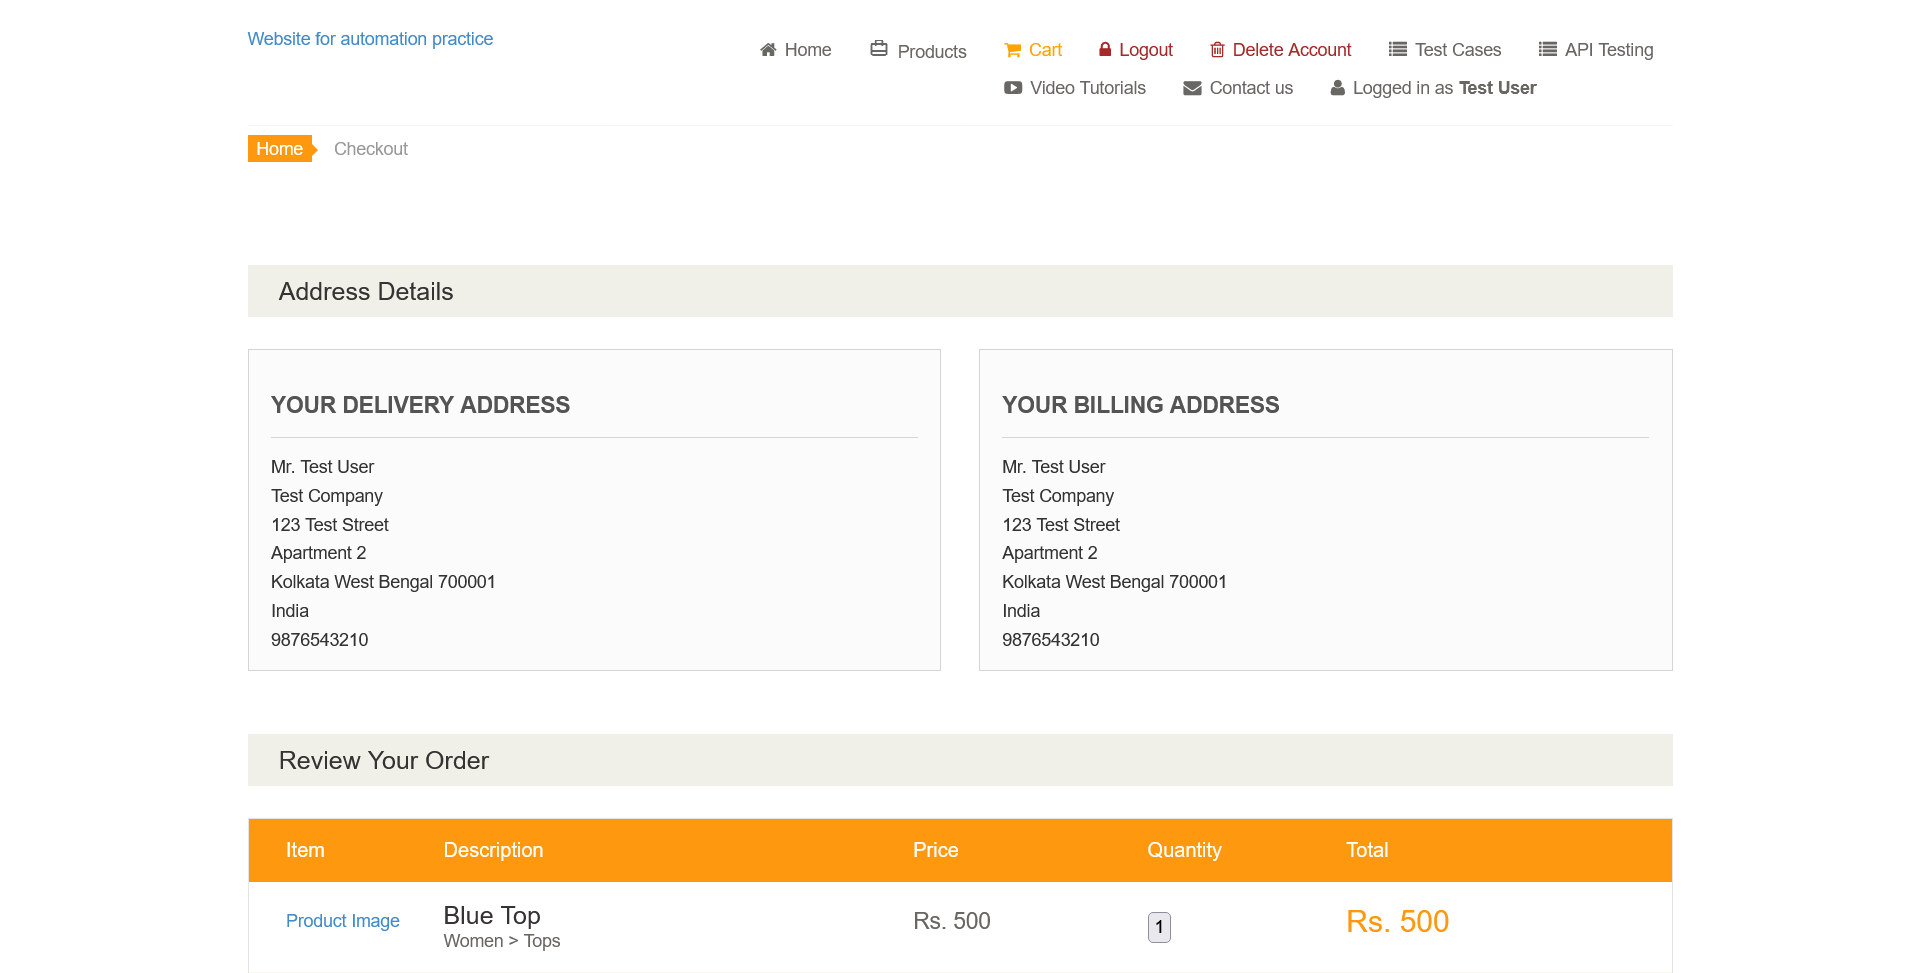
\includegraphics[width=0.76\textwidth]{checkout_page.png}
\caption{Checkout page.}
\end{figure}
\begin{figure}[H]\centering
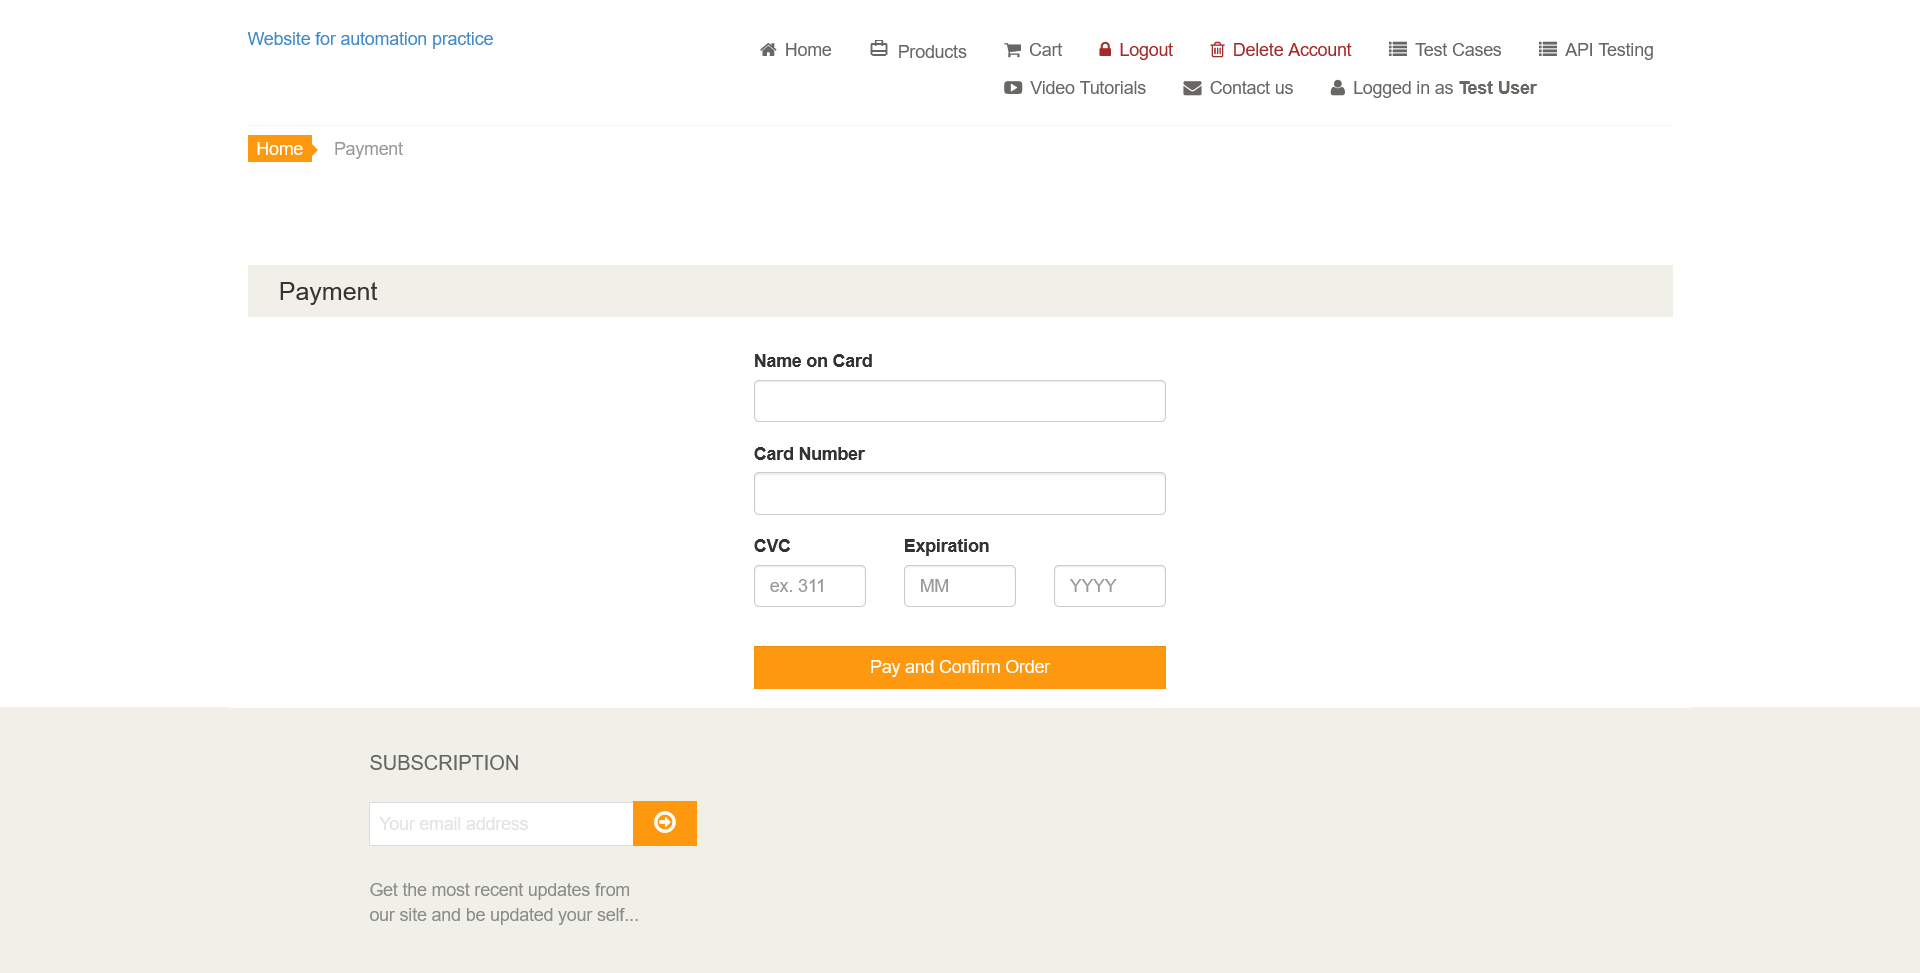
\includegraphics[width=0.76\textwidth]{payment_page.png}
\caption{Payment page.}
\end{figure}
\begin{figure}[H]\centering
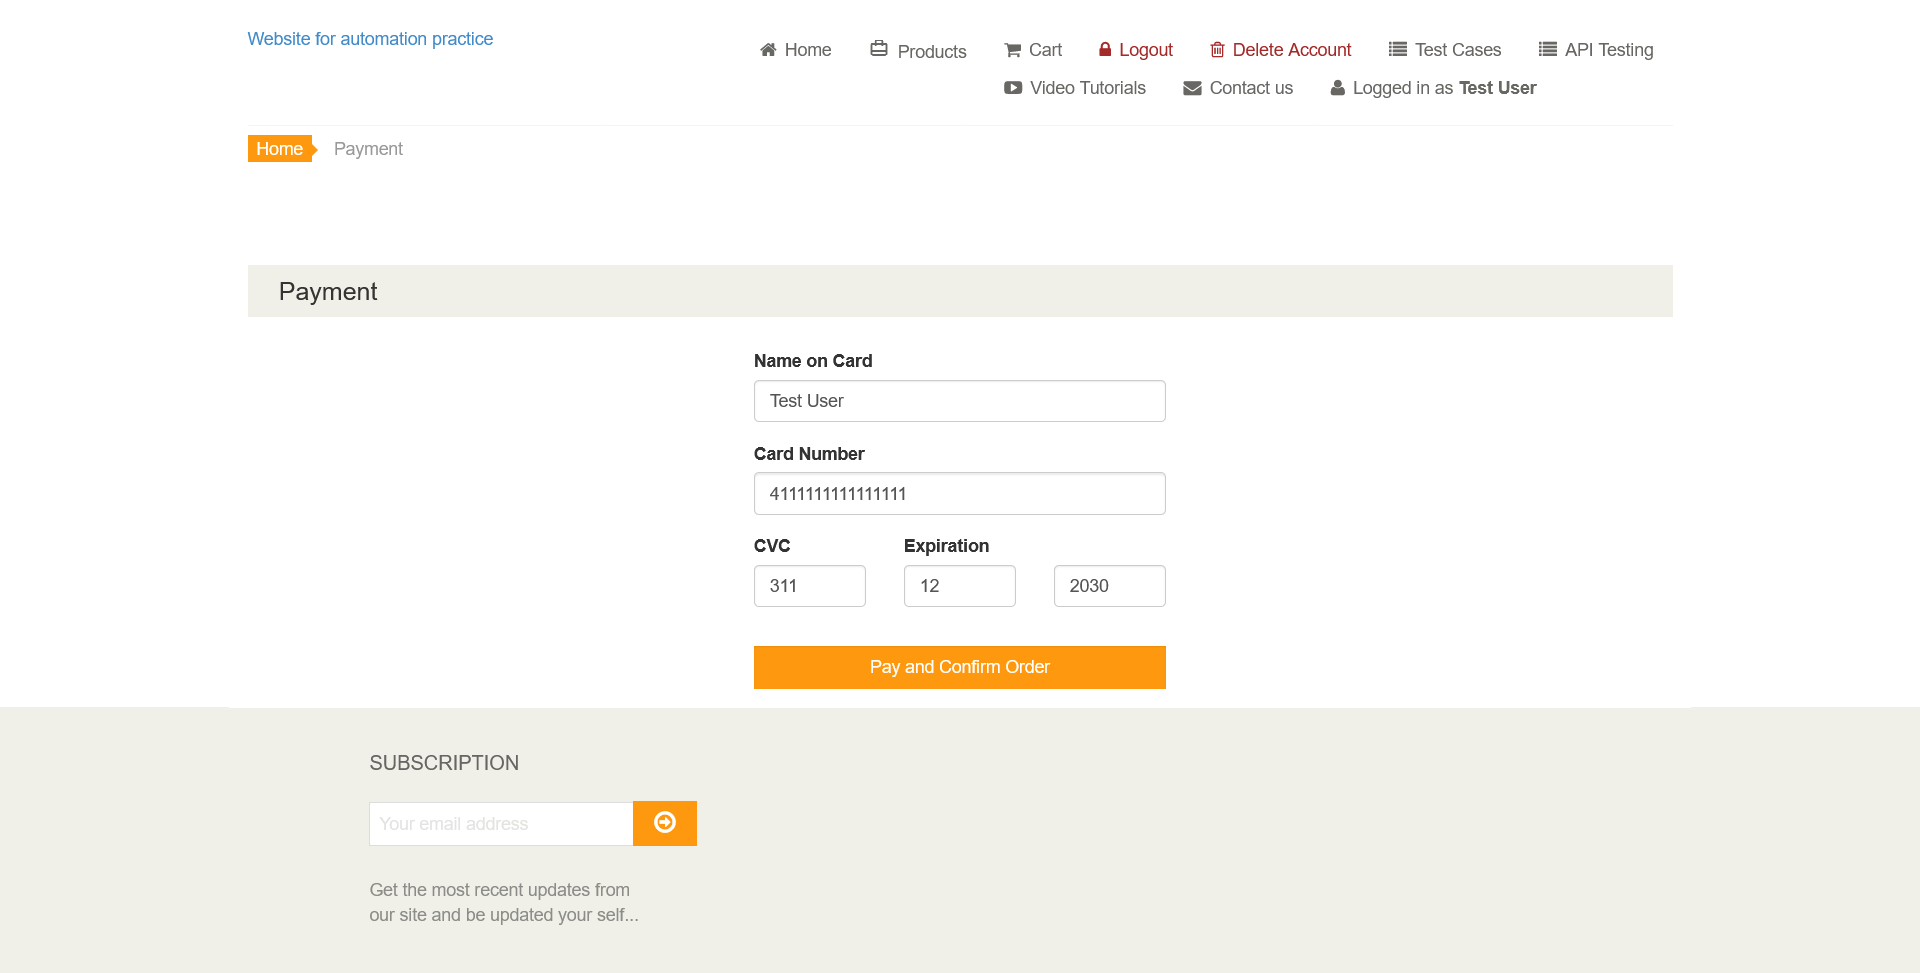
\includegraphics[width=0.76\textwidth]{payment_details.png}
\caption{Payment details entered.}
\end{figure}
\begin{figure}[H]\centering
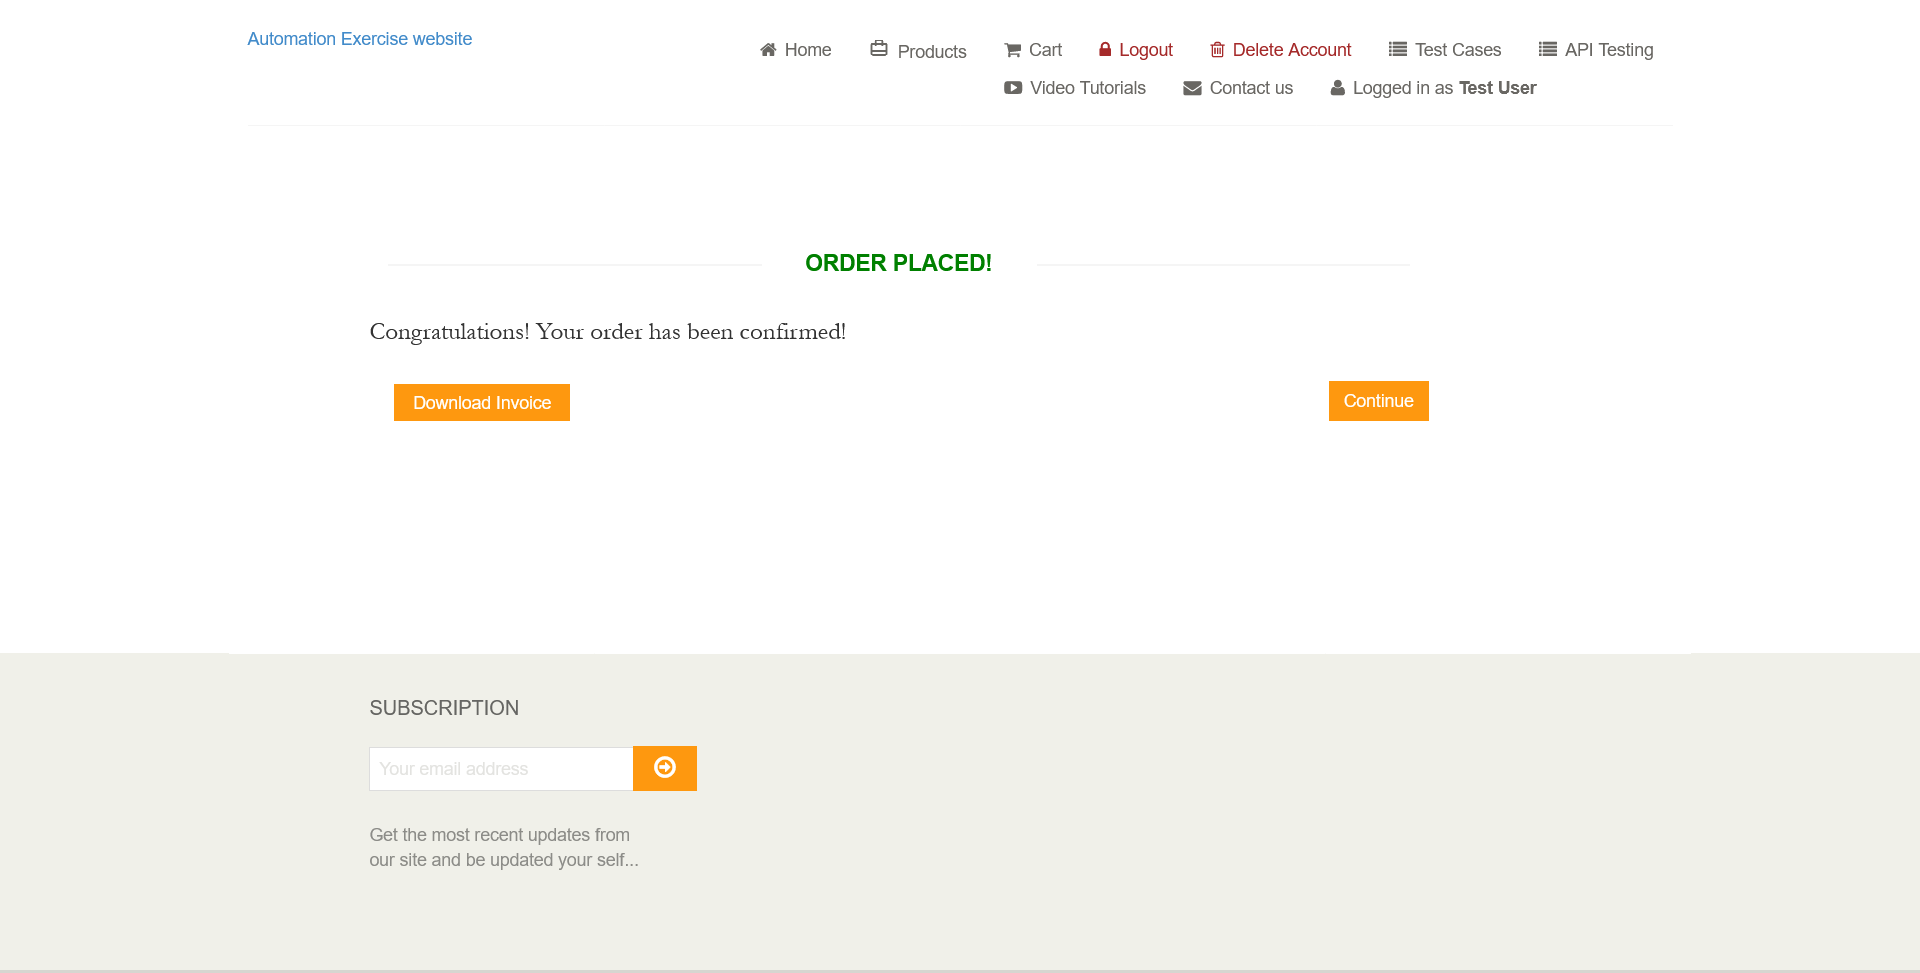
\includegraphics[width=0.76\textwidth]{order_success.png}
\caption{Order confirmation page.}
\end{figure}

% 21. Challenges Faced
\section{Challenges Faced}
The main challenge was advertisement overlays. Dynamic advertisement iframes can cover controls, intercept mouse clicks, and cause Selenium interactions to fail even when the target control exists. This is particularly relevant around signup, search, and product-card actions.

The project includes \texttt{remove\_ads(driver)} in \texttt{popup.py}. It runs JavaScript that removes iframe elements with common Google Ads and DoubleClick identifiers, names, or source URLs. The calls are currently commented out in the primary flow, so normal site behavior is preserved; they can be enabled before sensitive interactions if overlays recur. Other challenges include the timing of dynamic elements, reuse of an existing account, and reliance on the external demo website's changing page structure.

% 22. Advantages
\section{Advantages}
\begin{itemize}[leftmargin=1.6em]
  \item Automates a complete customer journey rather than isolated page actions.
  \item Uses reusable modules and external CSV/configuration data.
  \item Applies explicit waits to improve reliability on dynamic pages.
  \item Produces screenshots and logs that support troubleshooting and reporting.
  \item Supports both a Pytest-based test and a standalone execution route.
\end{itemize}

% 23. Limitations
\section{Limitations}
The project is tied to one demo website and its current UI locators. It does not yet use a formal Page Object Model, parameterized tests, test markers, reporting plugins, or a dependency manifest. Cart quantity values are present in the CSV file but are not applied. The flow does not validate cart totals, download invoices, or capture screenshots automatically on every failure. Test credentials and payment data are stored in plain text for demo purposes and must not be used for real accounts or real payment systems.

% 24. Future Scope
\section{Future Scope}
Future development can introduce page-object classes, a \texttt{requirements.txt} file, environment variables for sensitive data, parameterized positive and negative test cases, headless execution, HTML test reports, and CI/CD integration. The cart flow can be extended to update quantities from \texttt{products.csv}, validate prices and totals, handle coupon cases, verify final confirmation text, and download invoices. Failure handling can capture a screenshot and browser diagnostic data automatically for each failed action.

% 25. Conclusion
\section{Conclusion}
This project demonstrates a practical Selenium-based e-commerce automation solution. It uses Firefox and a shared WebDriver session to execute registration or login, product search, cart addition, checkout, payment, and final confirmation. CSV configuration, explicit waits, logging, and screenshots make the scenario repeatable and provide clear test evidence.

The implementation is a strong foundation for broader automated testing. Its next stage should focus on stronger assertions, cart validation, a formal Page Object Model, safer test-data handling, and CI-ready execution. The current workflow successfully illustrates how browser automation can validate a complete online purchase journey efficiently and consistently.

\end{document}
